\documentclass{article}
\usepackage[spanish]{babel}
\usepackage[utf8]{inputenc}
\usepackage{graphicx}
\usepackage[a4paper,top=1.5cm,bottom=1.5cm,left=2cm,right=2cm]{geometry}
\usepackage{caption,subcaption}
\usepackage{amsmath}
\usepackage{cancel}
\usepackage{natbib}
\title{Turbiedad}
\author{Lalih Otrebor feat. Cana Inalec}
\date{April 2019}
\usepackage{siunitx}
\graphicspath{ {fig/} }
\usepackage{bm}

\newcommand{\glossentry}[2]{$#1$\indent #2 \par \vspace{.4cm} }


%
\newcommand{\tita}{\theta}
\newcommand{\substy}[2]{\ensuremath{{#1_{\mathrm{#2}}}}}
\newcommand{\sib}[1]{\ensuremath{\left[\si{#1}\right]}}
\newcommand{\degree}{\ensuremath{{^\circ}}}
\newcommand{\attackangle}{{\ensuremath{\bm{\alpha}}}}
\newcommand{\cp}{c_p}
\newcommand{\cteuniversal}{\ensuremath{\tilde{R}}}
\newcommand{\molarmass}{\ensuremath{{\scriptstyle \bar{M}}}}
\newcommand{\Rconst}{R}
\newcommand{\gasconst}{k}
\newcommand{\ctegas}{\gasconst}
% \newcommand{\speedsound}{{c_{\!s\!}}}
\newcommand{\relative}{\mathrm{rel}}
\newcommand{\speedsound}{a}
\newcommand{\ctan}[1]{\ensuremath{c_{\theta #1}}}
\newcommand{\crad}[1]{\ensuremath{c_{r #1}}}
\newcommand{\cax}[1]{\ensuremath{c_{a #1}}}
\newcommand{\angvel}{\ensuremath{\omega}}
\newcommand{\Mach}{\textrm{M}}
\newcommand{\di}{\textrm{d}}
\newcommand{\cte}{\textrm{constante}}
%Entradas para glosario 
\newcommand{\etaiso}{\eta_{\mathrm{iso}}}
\newcommand{\Sgen}{\substy{S}{gen}}
\newcommand{\dQ}{\dot{Q}}
\newcommand{\dU}{\dot{U}}
\newcommand{\dW}{\dot{W}}
\newcommand{\dm}{\dot{m}}
\newcommand{\etaTot}{\substy{\eta}{iso}}
\newcommand{\etahid}{\substy{\eta}{h}}
\newcommand{\etamec}{\substy{\eta}{m}}
\newcommand{\slip}{\xi}
\newcommand{\deflectionangle}{{\vartheta}}
\newcommand{\slipangle}{\ensuremath{\theta_d}}
\newcommand{\radrel}{\nu}
\newcommand{\rext}{\substy{r}{ext}}
\newcommand{\rbase}{\substy{r}{base}}
\newcommand{\powerreduction}{\mu}
\newcommand{\degreeofreaction}{{\bm{R}}}
\newcommand{\relcomp}{\ensuremath{r_c}}
\begin{document}

\maketitle

\section*{Glosario}
Subíndice $1$ indica la entrada al rotor, $2$ indica salida del rotor, $B_s$ indica el estado $B$ para el proceso isoentrópico.
\par

\glossentry{\speedsound}{La velocidad del sonido en un fluido}


\glossentry{c}{Velocidad absoluta del fluido}
% \glossentry{\cax{}=V}{Velocidad axial del fluido}
\glossentry{\ctan{}}{Velocidad tangencial del fluido}
\glossentry{\cax{}}{Velocidad axial del fluido}

\glossentry{\crad{}}{Velocidad radial del fluido}
\glossentry{w}{Velocidad relativa del fluido con respecto al rotor}
\glossentry{U}{Velocidad del impulsor}
\glossentry{\cteuniversal=8,314 \si{\joule \per \kelvin\per \mole}}{Constante universal para gases ideales}
\glossentry{R=\molarmass\cteuniversal}{Constante especifica de un gas ideal \sib{\joule \per \kilogram \per \kelvin} donde \molarmass{} es la masa molar \sib{\kilogram \per \mole}}
\glossentry{\degreeofreaction}{Grado de reacción}
\glossentry{\relcomp}{Relación de compresión}
\glossentry{r,D}{Radio y diámetro, respectivamente}
\glossentry{\Mach=\frac{c}{\speedsound}}{Número de Mach}
\glossentry{\alpha}{Ángulo entre velocidad absoluta con respecto al plano meridional}
\glossentry{\attackangle}{Ángulo de ataque del alabe}
\glossentry{\beta}{Ángulo entre velocidad relativa con respecto al plano meridional}
\glossentry{\delta}{Ángulo de desviación del alabe o espesor de capa límite}
% \glossentry{\slipangle}{Ángulo de deslizamiento}
\glossentry{\psi}{Coeficiente}
\glossentry{\phi}{Coeficiente de flujo $\frac{\crad{2}}{U_2}$}
\glossentry{\slip}{Coeficiente de deslizamiento}
\glossentry{\Omega}{Velocidad angular del rotor}


\clearpage
% end of glossary
%------------------
\setcounter{section}{-1}

\section{Turbomaquinas}
Se clasifican como turbomaquinas todo dispositivo donde se transfiere energia desde o hacia un flujo continuo mediante la \textit{acción dinámica} de uno o mas alabes moviles. La fila de alabes moviles (rotor o impulsor) cambia la entalpia de estancamiento del fluido de trabajo haciendo trabajo positivo o negativo.

La palabra \textit{turbo} o \textit{turbinis} viene del latín e implica algo que da vueltas o gira. Hay varias formas de categorizar estas maquinas

\begin{enumerate}
    \item Segun su Grado de Reaccion ($\degreeofreaction$)
    \begin{itemize}
        \item De Accion: El cambio de presion ocurre sobre una tobera donde es dirigida hacia el rotor
        \item De Reaccion: La mayoria del cambio de presion ocurre sobre el rotor o impulsor
    \end{itemize}
    \item Direccion de flujo
    \begin{itemize}
        \item Tangenciales: Flujo incide tangencialmente sobre el rotor. Pelton es un ejemplo
        \item Axiales: Flujo es en su mayor parte paralelo al eje de rotación de la turbomaquina.
        \item Radiales: El flujo se contiene en el plano perpendicular al eje de rotación, principalmente acercándose o alejándose del eje.
        \item Mixtas: Componentes de velocidad mixta
    \end{itemize}
    \item Según sentido de transmision de energia
    \begin{itemize}
        \item Motoras: Turbinas
        \item Generadoras: Bombas, compresores, ventiladores
    \end{itemize}
    \item Según compresibilidad/tipo de flujo
    \begin{itemize}
        \item Térmicas
        \item Hidráulicas
    \end{itemize}
\end{enumerate}

\part{Primer Parcial}

\section{Leyes fundamentales de turbomaquinas}
Las leyes detalladas son totalmente generales y funcionan para flujos compresibles e incompresibles.
\begin{itemize}
    \item Continuidad
    \item La Primer Ley
    \item Conservacion de cantidad de movimiento
    \item La Segunda Ley
\end{itemize}
Se toma las siguientes hipotesis para el analisis de turbomaquinas
\begin{itemize}
    \item[H] Regimen estacionario
    \item[H] Cambio de energía potencial despreciable
\end{itemize}

La \textbf{gran} mayoría de los procesos con turbomaquinas se pueden considerar adiabáticos. La validez de esta hipótesis crece con el caudal másico y la velocidad. $\dQ=0$ 

\subsection{Continuidad}
Suponemos que la cantidad de masa en nuestra turbomaquina no varia durante su operación, por ende la cantidad de masa que entra es la misma que sale.
\[
\dm = \rho_1 c_1 A_{n_1} = \rho_2 c_2 A_{n_2} = \rho c A_n
\]
donde $c_i$ es la velocidad en dirección $n_1$, $A_{n_1}$ es la superficie normal a la dirección $n_1$.

\subsection{Primera Ley de la Termodinámica}
La primera ley de la termodinámica planteada entre dos puntos de un volumen de control es
\[
\dU = \dQ - \dW - \dm \left[\Delta h + \tfrac{1}{2}(c_2^2-c_1^2) + g(z_2 - z_1)\right]
\]
donde $h$ es la entalpía especifica, $c$ es la velocidad absoluta, $z$ es la altura del punto. Como se considera regimen estacionario $\dU=0$, ademas se suelen despreciar la energia potencial. Nos queda entonces el trabajo expresado en función de la entalpia y la energia cinetica.
\begin{equation} \label{ec:PrimeraLeyTurbomaquinas}
    \dW - \dQ = - \dm \left[ h_2-h_1 +\tfrac{1}{2}(c_2^2-c_1^2) \right] = - \dm (h_{02} - h_{01})
\end{equation}
por convenciencia se agrupan los terminos en la entalpia de estancamiento: $h_0 = h+\tfrac{1}{2}c^2$.

Puede ser mas conveniente escribir las ecuaciones en funcion si producen o entregan trabajo, asi el termino de trabajo siempre es positivo.
\begin{align*}
        \qquad \qquad \dW_t &= \dm (h_{01}-h_{02}) \quad \text{Para turbinas adiabáticas ($\dW>0$)} \\
        \dW_c &= \dm (h_{02}-h_{01}) \quad \text{Para compresores y bombas adiabáticos ($\dW<0$)} 
\end{align*}

\subsection{Conservación de la cantidad de momento angular}


\begin{figure}[ht!]
    \centering
    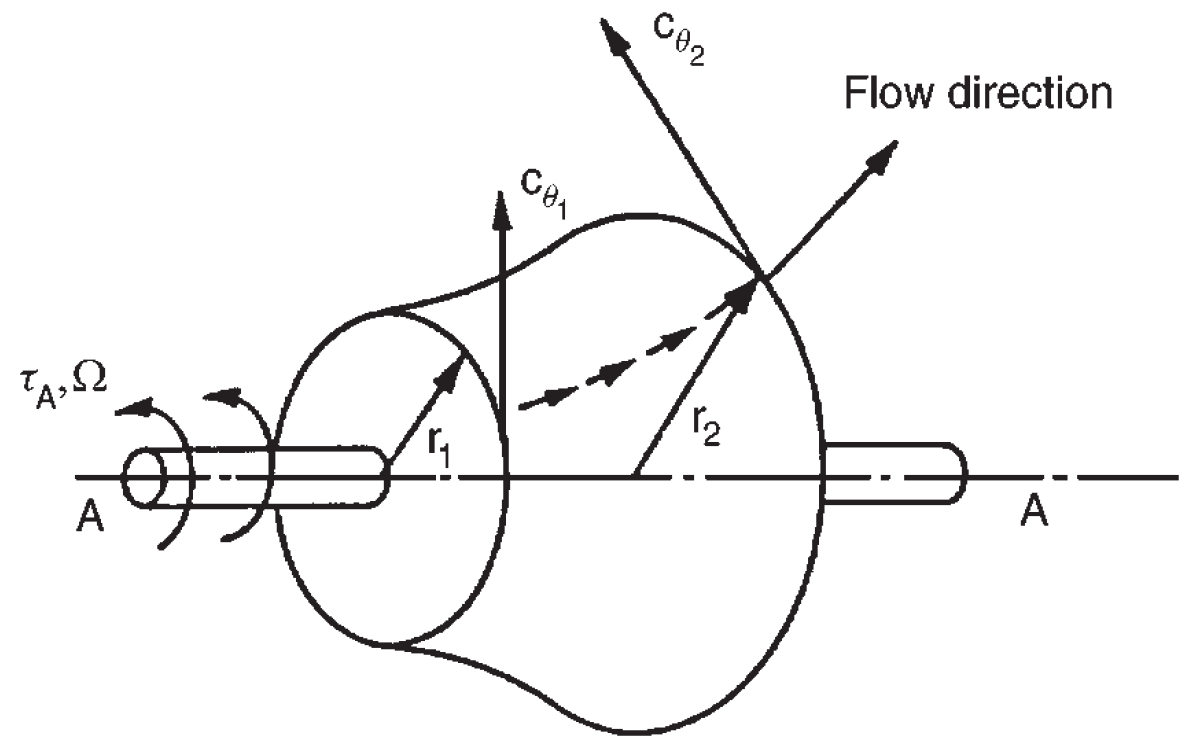
\includegraphics[width=9cm]{fig/turb.png}
    \caption{Esquema generalizado de una turbomaquina. $\Omega=\angvel,\quad$      $\tau_A=\dot{m}(r_2 \ctan{2} -r_1 \ctan{1}$)}
    \label{fig:turbina}
\end{figure}
Para un sistema de masa $m$, la suma vectorial de todos los momentos de las fuerzas externas (torque del eje para turbomaquinas) que actuan sobre un eje arbitrario A--A (fijo en el espacio) es igual  a la razón de cambio de la velocidad angular del sistema sobre ese mismo eje.

\[
\tau_{A} = m \frac{\di}{\di t} (r \ctan{})
\]
donde $r$ es la distancia entre el centro de masa y el eje A. $\ctan{}$ es la velocidad de la masa mutuamente perpendicular al vector de radio $r$ y el eje A. 

Para un volumen de control en régimen estacionario (figura \ref{fig:turbina}) se expresa el cambio de momento angular entre dos puntos:

\begin{equation}\label{eq:eulerparaTubomaquinas}
    \tau_{A}= \dot{m} (r_2\ctan{2} -r_1 \ctan{1})  \quad \Rightarrow\quad \dW =\dm (U_2 \ctan{2}- U_1 \ctan{1})  
\end{equation}
donde $\Omega$ es la velocidad angular; $U=\omega r$ es la velocidad del alabe. Recordar que $\dW = \Omega \tau$.


Una de las consecuencias útiles es que si se aplica el teorema del coseno a la figura \ref{fig:veltrianggeneral} se tiene que

\[
w^2 = U^2 +c^2 -2U c \cdot \cos \theta 
\]
por ende tenemos que $Uc\cdot \cos \theta = (w^2-U^2-c^2)/2$, resultando en la ecuación expandida de Euler \ref{eq:eulerexpanded}

\begin{equation} \label{eq:eulerexpanded}
    \frac{\dot{W}}{\dot{m}}=e= \left(\frac{c_2^2-c_1^2}{2}\right)+\left(\frac{U_2^2-U_1^2}{2}\right)+\left(\frac{w_1^2-w_2^2}{2}\right)
\end{equation}
Se puede interpretar los terminos con $c$ y $w$ como la potencia aerodinamica y el termino con $U$
\subsection{Segunda Ley de la Termodinámica}
Por alguna razón (Enunciado de Clausius) establece que para un sistema recorriendo un ciclo

\[
\oint \frac{\di Q}{T} \leq 0
\]
La cantidad que se obtiene con el integral se denomina \textit{entropía}. Para un ciclo reversible dicha integral da cero.

\[
S_2 - S_1 = \int^2_1 \frac{\di Q}{T}
\]

Para un sistema en régimen estacionario
\[
\int^2_1 \frac{\di\dot{Q}}{T} \leq \dot{m}(s_2 -s_1)
\]
si el proceso es adiabático $\di \dot{Q}=0$ entonces $s_2\geq s_1$.  Si el proceso además es reversible también entonces $s_2 =s_1$.

Esto sale de la igualdad de termodinámica
\[
\cancelto{\textrm{Adb.}}{\Delta S_0} + \cancelto{\textrm{Iso.}}{\Delta S} = \cancelto{\textrm{Rev.}}{\Sgen} \geq 0
\]



\section{Ecuaciones de gas compresible}
Definimos $\cteuniversal=8,314$ \si{\joule \per \kelvin\per \mole} como la constante universal de gases tal que $\cteuniversal = \frac{R}{\molarmass}$ donde $\molarmass$ es la masa molar.
\begin{figure}[htb!]
\centering
\begin{subfigure}{.49\textwidth}
\centering
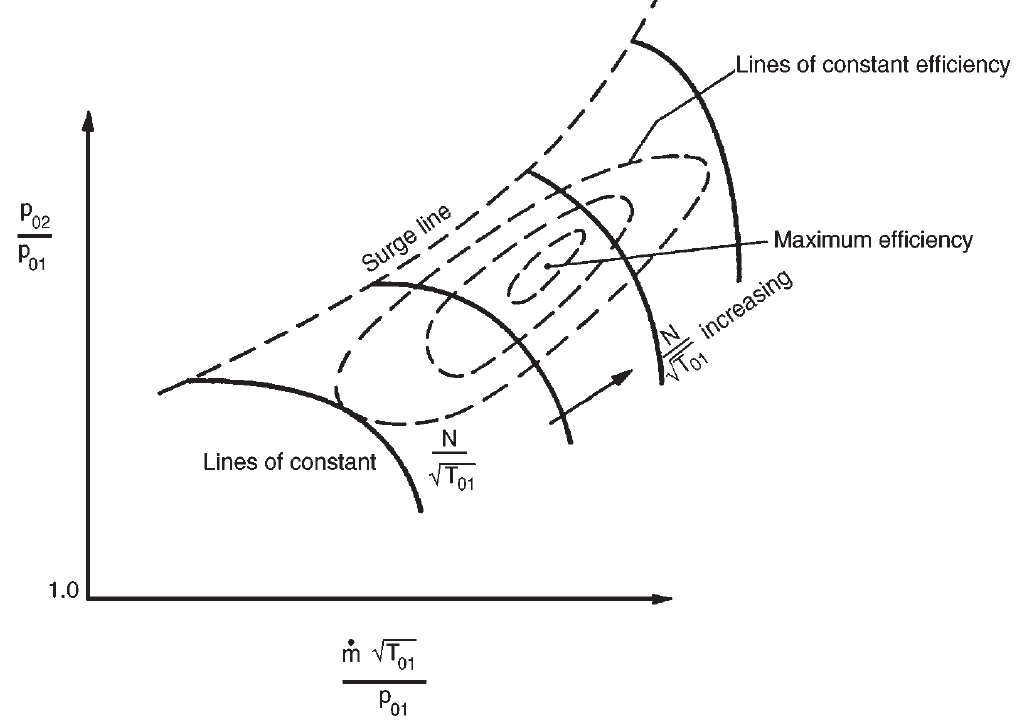
\includegraphics[height=6cm]{fig/caracteristicascompresor.png}
\caption{Compresor}
\label{fig:caractcompresor}
\end{subfigure}%
\begin{subfigure}{.49\textwidth}
\centering
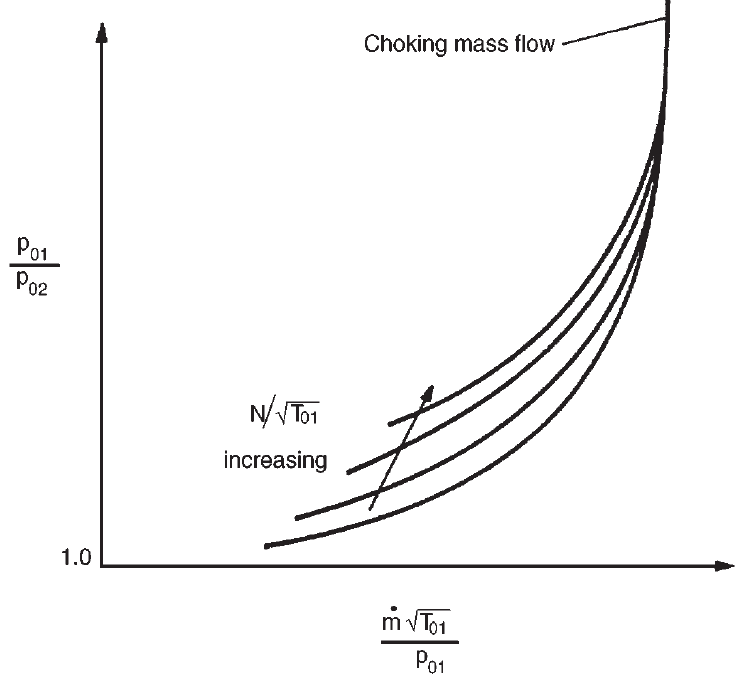
\includegraphics[height= 6cm]{fig/caracteristicasturbina.png}
\caption{Turbina}
\label{fig:caractturbina}
\end{subfigure}
\caption{Características de turbomáquinas.}
\label{fig:caracteristicasturbomaquinas}
\end{figure}
\subsection{Entalpía de estancamiento} 
Constante para un proceso que no involucra transferencia de trabajo o transferencia de calor aunque si pueden estar presentes procesos irreversibles.
\[
h_0 = h+\tfrac{1}{2}c^2
\]
si el fluido es gas perfecto \( h=\cp T\) donde \( \cp = \gasconst \Rconst (\gasconst-1)^{-1} \).
\[
T_0 = T + \tfrac{1}{2}\frac{c^2}{\cp}
\]

\begin{equation}\label{eq:tempstagnation}
 \frac{T_0}{T}=1+\tfrac{1}{2}(\gasconst-1)\frac{c^2}{\gasconst\Rconst T}=1+\tfrac{1}{2}(\gasconst-1)\Mach^2
\end{equation}
La relación de Gibbs derivada de la segunda ley:
\[T\di s = \di h - \frac{1}{\rho}\di p
\]
si el fluido es traído al reposo mediante un proceso adiabático y reversible entonces

\[\di h = \cp \di T =\frac{\di p}{p}\Rconst T
\]
tal que
\[
\frac{\di p}{p} = \frac{\cp}{\Rconst}\frac{\di T}{T} = \frac{\gasconst}{\gasconst-1}\frac{\di T}{T}
\]
integrando obtenemos
\[
\ln p = \ln \cte + \frac{\gasconst}{\gasconst-1}\ln T
\]
por ende
\begin{equation}
    \frac{p_0}{p}=\left(\frac{T_0}{T} \right)^{\frac{\gasconst}{\gasconst-1}} =\left(1+ \frac{\gasconst-1}{2}\Mach^2 \right)^{\frac{\gasconst}{\gasconst-1}}
\end{equation}
y de la ley de gases ideales sabiendo que \(\rho = p/(RT)=\frac{1}{v} \)


\begin{equation}
    \frac{\rho_0}{\rho}=\left(\frac{T_0}{T} \right)^{\frac{1}{\gasconst-1}} =\left(1+ \frac{\gasconst-1}{2}\Mach^2 \right)^{\frac{1}{\gasconst-1}}
\end{equation}
\[
\Mach=\frac{c}{\speedsound} = \frac{c}{\sqrt{\gasconst \Rconst T}}
\]
\subsection{Ecuaciones de Euler para bombas y turbinas}

La ecuación de Euler es un modelo para el torque y la potencia de una turbomáquina. Utiliza el flujo másico, la velocidad angular y la geometría. Se obtiene a partir de la conservación de momento angular. 

\subsection*{Triángulo de velocidades} Para el estudio del flujo en el interior de una turbomáquina se define la velocidad de flujo $\Vec{c}$ absoluta, la velocidad de flujo relativa $\Vec{w}$\footnote{En el estudio de turbomaquinas es conveniente plantear un marco de referencia sobre el rotor. En este marco de referencia se esta operando en régimen estacionario.} y la velocidad del sistema móvil $\Vec{U}=\Omega \times r$ y los ángulos $\alpha$, $\beta$ y $\theta$. Los distintos libros usan distintas letras para los ángulos, lo que hace que las ecuaciones se vean distintas. Aquí se toman los nombres usados por Dixon, que figura en \ref{fig:veltrianggeneral}. 

El triángulo de velocidades no es más que la aplicación de los principios de mecánica General: 

\[\Vec{c}=\Vec{U}+\Vec{w}\]

Parado en el sistema móvil, donde las paletas están fijas, se observaría que el flujo es tangente a la paleta. Por eso en los triángulos de velocidades se debe dibujar $\Vec{w}$ en esa dirección. Quedan relacionadas las velocidades con los ángulos de ataque y de fuga del diseño.

\begin{figure}[htb!]
    \centering
    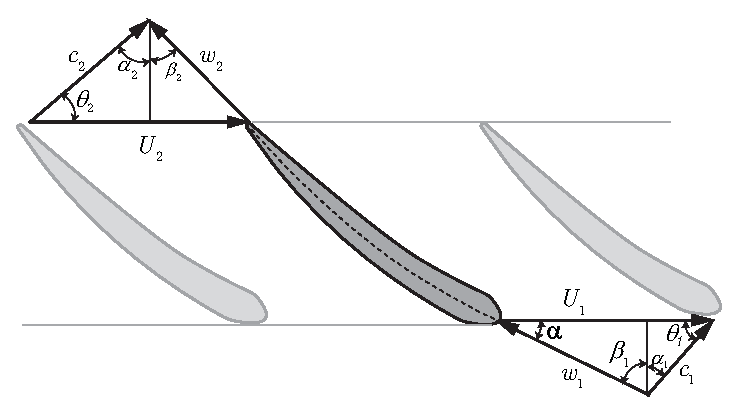
\includegraphics[width=0.6\textwidth]{fig/VelTrianglegeneral.eps}
    \caption{Triangulo de velocidades para un alabe de un rotor de un compresor axial. Gira en sentido de $U$.}
    \label{fig:veltrianggeneral}
\end{figure}

\subsubsection*{Continuidad o Conservación de la masa}
Si el enunciado no informa acerca de las velocidades, éstas se pueden relacionar con el flujo másico teniendo en cuenta que la materia que ingresa es la misma que la que sale (tanto en el sistema absoluto como en el móvil).

la ecuación tiene la forma de 
\[
\dm=\rho_1 A_1 c_{n1} = \rho_2 A_2 c_{n2}
\]

donde $c_{ni}$ es la velocidad del fluido en dirección normal a la superficie de área $A_i$. En turbinas axiales la velocidad $c_{n}$ no es otra que $c_{a}$, y se suele constante en el álabe porque el cambio de densidad no es pronunciado. 







\section{Definiciones de eficiencias}
Según la primera ley de la termodinámica tenemos que el cambio en la energía interna esta dada por
\begin{equation}
    \dot{U} =\dQ -\dW = \dm \left[(h_2-h_1)+\tfrac{1}{2}(c_2^2-c_1^2)+g(z_2-z_1) \right]
\end{equation}
Como la mayoría de las turbomáquinas se aproximan a ser adiabáticas y que los cambios en energía potencial son insignificantes en la gran mayoría de los casos llegamos a
\begin{equation}
    \dW = \dm \left[ h_1+\tfrac{1}{2}c_1^2 - (h_2+\tfrac{1}{2}c_2^2) \right] = \dm \left( h_{01}-h_{02}\right)
\end{equation}

para compresores (absorben energía) es más conveniente escribir
\[
\dW_c=-\dW =\dm \left( h_{02}-h_{01}\right)
\]

Un trayecto sin intercambio de trabajo para flujos incompresibles y flujos compresibles isoentrópico la presión de estancamiento es constante
\[
p_{01}=p_{02}=p_0=\cte
\]
$p_0$ siendo la presión de estancamiento $p_{0}=p+\tfrac{1}{2} \rho c^{2}$.
\subsection{Eficiencia}
La eficiencia total:
\[
\etaTot  = \frac{\textrm{Potencia mecánica disponible a la salida del eje}}{\textrm{Máxima diferencia de energía posible en el fluido por unidad tiempo}}
\]
LA eficiencia isotentrópica o hidraulica:
\[
\etaiso=\etahid = \frac{\textrm{Potencia mecánica suministrada al rotor}}{\textrm{Máxima diferencia de energía posible en el fluido por unidad tiempo}}
\]
La eficiencia mecánica:
\[
\etamec = \frac{\etaTot}{\etaiso}
\]

Para un flujo incompresible, en la ausencia de fricción se tiene que la potencia máxima que se puede obtener de una turbina es
\[
\dW_{\max} = \dm  \left[ (h_{01}-h_{02s})+g(z_1-z_2) \right]= \dm g \left(H_1-H_2 \right)
\]
donde $gH = \frac{p}{\rho}+\frac{1}{2}c^2+gz$.

\begin{figure}[htb!]
\centering
\begin{subfigure}{.49\textwidth}
\centering
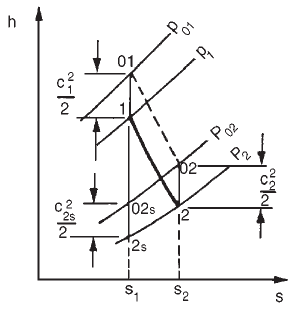
\includegraphics[height=6cm]{fig/expansionturbina.png}
\caption{Proceso de expansión en una turbina}
\label{fig:expansiontrubina}
\end{subfigure}%
\begin{subfigure}{.49\textwidth}
\centering
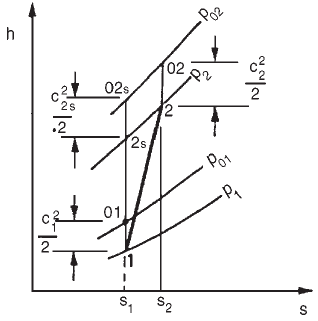
\includegraphics[height= 6cm]{fig/procesocompresion.png}
\caption{Proceso de compresión }
\label{fig:procesocompresion}
\end{subfigure}
\caption{Diagramas $h$--$s$ para turbinas y compresores}
\label{fig:procesosturbomaquinasHS}
\end{figure}



\section{Compresores centrífugos}


El borde del inductor debe tener el mismo ángulo que tiene la velocidad relativa del fluido ($\beta_1$) al entrar en la bomba y así evitar el choque entre inductor y fluido. Para un fluido sin prerotación:
\[
\tan \beta_1 = \frac{\cax{1}}{U_1}
\]

\subsection{Choke o estrangulamiento}
El punto de estrangulación es el máximo caudal que admite
la maquina a una cierta velocidad de giro.   
El fenómenos de estrangulación se da cuando en la mínima
sección de paso del gas este alcanza la velocidad del sonido,
produciendo tantas perdidas que se convierte en el punto
máximo de caudal.
Este fenómeno no afecta la vida del compresor sin embargo
limita el campo de operación del mismo.

\subsection{Deslizamiento}
Aún en condiciones ideales con alabes sin fricción el flujo es impulsado de manera imperfecta por los alabes debido a la aceleración de Coriolis. Se dice que el fluido \textit{desliza}. Se podría pensarlo como una diferencia de presión entre las dos superficies de un alabe dando luz a una velocidad relativa en dirección opuesta a la rotación. El efecto aumenta con la luz entre alabes, por ende se necesita un número \textbf{infinito} de alabes para que no haya deslizamiento.

\begin{figure}[htb!]
\centering
\begin{subfigure}{.49\textwidth}
\centering
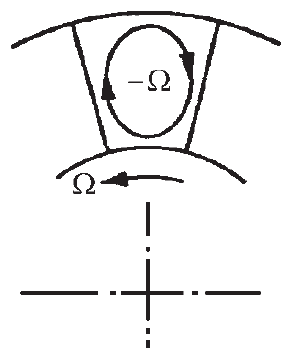
\includegraphics[height=5cm]{fig/eddydeslizamiento.png}
\caption{Eddy relativa formada por haber finitos alabes}
\label{fig:deslizamientoEddy}
\end{subfigure}%
\begin{subfigure}{.49\textwidth}
\centering
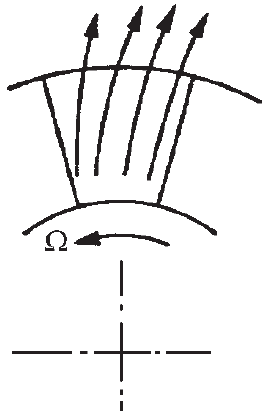
\includegraphics[height= 5cm]{fig/deslizamientoconeddy.png}
\caption{Flujo ideal sumado con eddy}
\label{fig:deslizamientoEddyMasFlujoIdeal}
\end{subfigure}
\caption{Visualización del deslizamiento}
\label{fig:explicaciondeslizamiento}
\end{figure}

\subsection{El coeficiente de deslizamiento}
Todas las velocidades son a la salida del rotor. El coeficiente de deslizamiento:
\[
\slip = \frac{\ctan{d}}{\ctan{}} = \frac{\ctan{}-u_d}{\ctan{}}
\]

Un estimativo de la velocidad de deslizamiento $u_d= \ctan{}-\ctan{\mathrm{deslizando}}$ sale de suponer que los eddys tienen el diámetro igual al espacio entre alabes $D_{\mathrm{eddy}}= \pi D_{\mathrm{2}}/Z$ donde $Z$ es el número de alabes. 
\[
u_d \sim \Omega \cdot \frac{D_{\mathrm{eddy}}}{2}
\]
donde $\ctan{}$ es la velocidad obtenida con la ecuación de Euler que no toma en cuenta el deslizamiento. El ángulo que se desvía el flujo por causa del deslizamiento:
\[
\tan (\beta_d) =\frac{\ctan{}-\ctan{d}}{\crad{}}= \frac{u_d}{\crad{}}
\]

Stodola (1927) propone una correlación para alabes curvos donde $\beta_2$ es el ángulo del alabe a la salida del rotor respecto la radial.

\[
D_{\mathrm{eddy}}\simeq \frac{\pi D_2\cos \beta_2}{Z} \quad\Rightarrow \quad \slip_{\mathrm{Stodola}} = 1-\frac{\pi \cos \beta_2}{Z(1-\phi_2 \tan \beta_2)}
\]
donde $\phi_2 =\frac{\crad{2}}{U_2}$.

Correlación Wiesner--Busemann (1967) (``la mejor", Se aproxima a la realidad):
\[
\ctan{d} =\frac{U_2\sqrt{\cos \beta_2}}{Z^{0,7}}
\quad\Rightarrow\qquad
\slip_{\mathrm{w}} = 1 - \frac{\sqrt{\cos \beta_2}}{Z^{0,7}(1-\phi_2\tan \beta_2)}
\]

\begin{figure}[htb!]
    \centering
    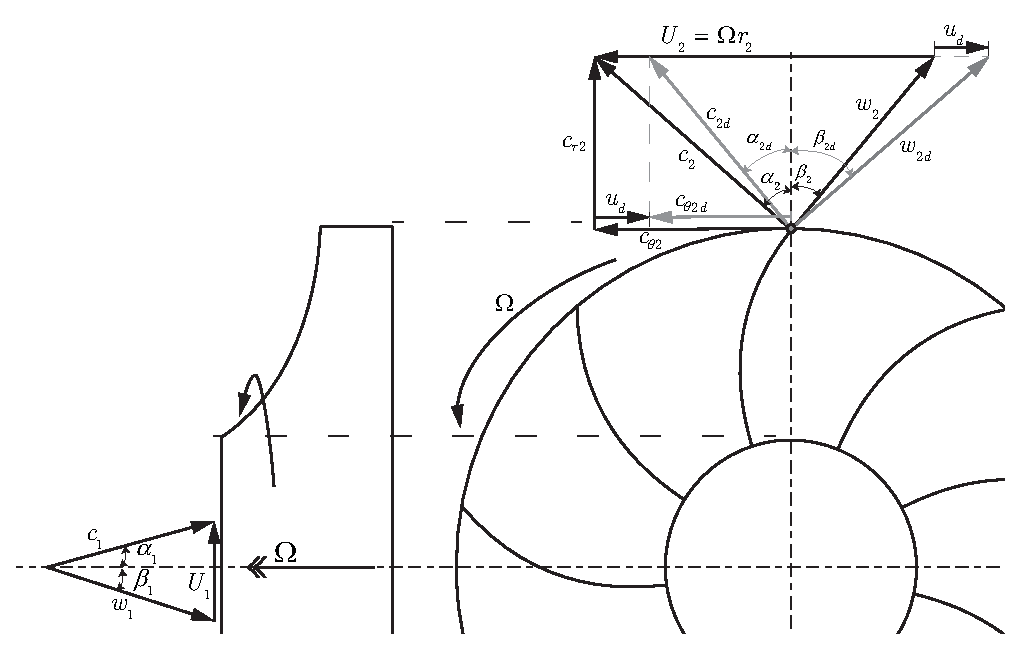
\includegraphics[width=0.7\textwidth]{fig/centrifugoVelocityTriangle.eps}
    \caption{Triángulos de velocidad para una bomba centrifuga con alabes curvados hacia atrás y con pre-rotación $\alpha_1$ positiva. }
    \label{fig:my_label}
\end{figure}
\subsection{Consideraciones del deslizamiento}
Potencia especifica:
\[
\frac{\dW_d}{\dm}=e_d = h_{02}-h_{01}=\ctan{2d} U_2 - \ctan{1} U_1 = (\slip \ctan{2})U_2 - \ctan{1} U_1
\]

\[
T_{03}-T_{01} = \frac{\slip \ctan{2}U_2-\ctan{1}U_1}{\cp}
\]

\[
\etaiso = \frac{\dW_{\mathrm{iso}}}{\dW_{\mathrm{real}}} = \frac{h_{03s}-h_{01}}{h_{03}-h_{01}}= \frac{T_{03s}-T_{01}}{T_{03}-T_{01}}
\]

\[
\frac{p_{03}}{p_{01}}= \left( \frac{T_{03s}}{T_{01}}\right)^{\frac{\ctegas}{\ctegas-1}} =\left[ 1+ \frac{\etaiso (\slip \ctan{2}U_2 - \ctan{1}U_1)}{\cp T_{01}} \right]
\]

Según valores experimentales el número de Mach ($\Mach$) no puede superar $0,9$ en el inductor. Para una entrada netamente positiva:
\[
\Mach_1 = \frac{\cax{1}}{\speedsound} = \frac{\cax{1}}{\sqrt{\ctegas R T_1}}
\]

En la salida del rotor se permite que el número de Mach sea similar a 1. Suele ser buena practica limitar $\crad{2}$ a ser menor a $\speedsound$,
\[
\Mach_2 = \frac{c_{2d}}{\sqrt{Z_2\ctegas R T_2}}
\]
donde $Z_2$ es el factor de compresibilidad del gas.


\subsection{Difusor}
\newcommand{\equis}{{\ensuremath{x}}}
Conservación de la cantidad de movimiento angular especifica para un punto \equis{} del difusor 
\[
\ctan{2} r_2 = c_2 r_2 \sin \alpha_2= c_\equis r_\equis \sin \alpha_\equis  = \cte
\]
por conservación de la masa
\[
\dm = \rho_2 A_2 \crad{2}  = (2\pi r_2 b_2 )(c_2 \cos \alpha_2) \rho_2 = (2\pi r_\equis b_\equis )(c_\equis \cos \alpha_\equis) \rho_\equis =\cte 
\]
donde $b_2$ es el alto de la salida del rotor. Nos  queda que $\tan \alpha_\equis=\cte$ para un fluido \textit{incompresible}, $\rho_\equis = \cte$.
\subsection{Análisis dimensional para compresores dinámicos}
Dos turbomáquinas son dinámicamente semejantes cuando el vector velocidad es geométricamente similar o paralelo en todos los puntos y con módulos proporcionales.
\begin{align}
    \pi_1 &= \frac{p_{02}}{p_{01}}\\
    \pi_2 &= \dm\frac{\sqrt{R T_{01}}}{D^2 P_{01}}\\
    \pi_3 &= \frac{\Omega}{\sqrt{RT_{01}}}\\
    \pi_4 &= \etaTot
\end{align}

\section{Compresores Axiales}
Se define la relación de radios

\[
\radrel = \frac{\rext}{\rbase}
\]

Se tiene que $U_1=U_2=U$ a lo largo del alabe. Además se diseñan para que la velocidad axial sea constante $\cax{1}=\cax{2}=\cax{}$. con estas hipótesis:
\[
\frac{\dW}{\dm}=U \cax{} (\cos \beta_2 - \cos \beta 1 )
\]

Un escalonamiento entre entrada al rotor y salida del estator nos dará un aumento de presión. Si se puede considerar que la densidad permanece constante (es razonable dado que el incremento en presión suele ser muy reducido en turbocompresores axiales) entonces el proceso es isoentrópico
\[
T\di s = \di h - v \di p =0\quad \Rightarrow \quad h_3 - h_1 = \frac{p_3-p_1}{\rho}
\]

Factor diminución de potencia
\[
\powerreduction = \frac{\Delta \substy{T}{real}}{\Delta \substy{T}{euler}} \quad \text{tal que} \quad \substy{\dW}{real} = \powerreduction \dW
\]

\[
\frac{p_{03}}{p_{01}} = \left[1 + \frac{\etaiso \powerreduction}{\cp T_{01}}U \cax{} (\cos \beta_2 - \cos \beta_1) \right]^{\frac{\ctegas}{\ctegas-1}}
\]
grado de reacción:
\[
\degreeofreaction = \frac{h_2 - h_1}{h_3 - h_1}
\]
en caso de $\rho = \cte$ se convierte en el salto de presiones entre rotor y estator.
\begin{figure}[htb!]
    \centering
    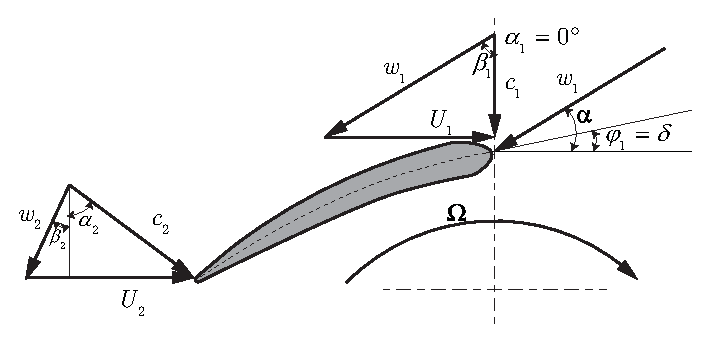
\includegraphics{fig/pumpVelTriangle.eps}
    \caption{Triangulo de velocidades para rotor de compresor axial con velocidad de entrada netamente axial $\alpha_1 = 0\degree$. Nomenclatura de \cite{book:TurboDick} }
    \label{fig:velocitytrianglepump}
\end{figure}

\section{Maquinas de despazamiento positivo}





\section{Ebullición}

\part{Segundo Parcial}

Parcial 2

aceite enfriado con intercambiador de calor

Anillo de lubricación: No muy bueno, para baja potencia.

ASTM D-445

Porque no uso mayor viscosidad? Consumis mas potencia para moverlo, pero aun mas importante no se produce una cuña hidrodinamica.

82 grados oxida aceite cojinetes
120 C fallan bubits

\section{Turbinas Hidraulicas}

El \textbf{rodete} es el elemento esencial de la turbina, estando provisto de álabes en los que tiene lugar
el intercambio de energía entre el agua y la máquina.

El \textbf{distribuidor} es un órgano fijo cuya misión es dirigir el agua, desde la sección de entrada de la
máquina hacia la entrada en el rodete, distribuyéndola alrededor del mismo, (turbinas de admisión
total), o a una parte, (turbinas de admisión parcial), es decir, permite regular el agua que entra en
la turbina, desde cerrar el paso totalmente, caudal cero, hasta lograr el caudal máximo. Es también
un órgano que transforma la energía de presión en energía de velocidad; en las turbinas
hélicocentrípetas y en las axiales está precedido de una cámara espiral (voluta) que conduce el agua
desde la sección de entrada, asegurando un reparto simétrico de la misma en la superficie de
entrada del distribuidor.

Las turbinas estas pueden tener un difusor o un escape libre.

En turbinas de \textbf{accion} el agua sale del distribuidor a presion atmosferica, impartiendo su energia cinetica al rodete.

el agua sale del distribuidor con
una cierta presión que va
disminuyendo su energia(presion y cinetica) a medida que el
agua atraviesa los álabes del
rodete, de forma que, a la salida, la
presión manometrica puede ser
nula o incluso negativa.

En las turbinas de acción, el empuje y la
acción del agua, coinciden, mientras que en
las turbinas de reacción, el empuje y la acción
del agua son opuestos

\begin{itemize}
    \item Axiales (Kaplan, helice, Bulbo)
    \item Radiales (francis)
    \item Tangenciales (Pelton)
    
\end{itemize}
Potencia de turbina de reaccion
\[
\frac{\gamma \mathrm{Q} \mathrm{u}\left(\mathrm{w}_{1} \cos \beta_{1}-\mathrm{w}_{2} \cos \beta_{2}\right)}{g}
\]

Eficiencia turb. reaccion 
\[
\phi=\frac{u}{(2 g H)^{1 / 2}}
\]
\subsection{Pelton}
Estas famosas turbinas tangenciales 

\subsubsection{Triangulo de velocidades}
Las paletas o cazoletas de estas turbinas tienen un parametro distintivo de construccion que es el angulo de defleccion, en la figura \ref{fig:peltontriangle} aparece como $\deflectionangle$, el cual suele estar contenido entre 140-170. 

Comob bien sabemos la potencia para una turbina esta dada por la ecuacion fundamental, y para una turbina Pelton tiene la forma ($U$ considerada igual en todo punto)
\[
\dot{W} = \dot{m} U (\ctan{1}-\ctan{2})=\dot{m} U (c_{1}-\ctan{2})
\]
donde $\ctan{2}$ se puede obtener usando la aproximación $U\approx w_2$ sabiendo que $c_2^2=w_2^2+U^2-2Uw_2\cos (\beta_2)$ nos queda
\[
c_2 \approx 2U\sin \frac{\beta_2}{2} 
\]
donde $\beta_2 = \pi - \vartheta_2 $. Por ende $\ctan{2} = c_2 \cos \theta_2$. Si se opta por la aproximación mencionada anteriormente entonces $\theta_2 \approx \frac{\vartheta_2}{2}$.

\begin{figure}[htb!]
    \centering
    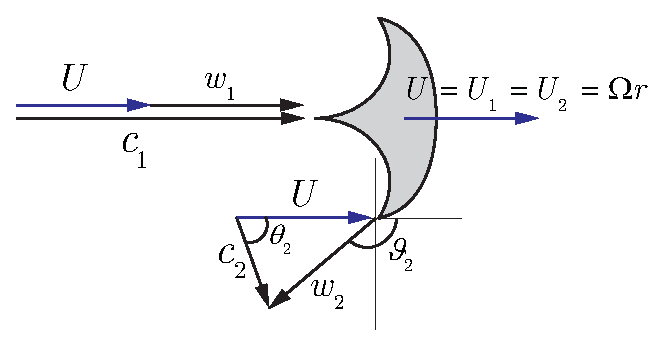
\includegraphics[width=0.5\textwidth]{fig/pelton_triangle.eps}
    \caption{Triangulo de velocidades para una turbina pelton.}
    \label{fig:peltontriangle}
\end{figure}

\subsubsection{Eficiencia}
La energia maxima que se puede aprovechar de la turbina Pelton esta dada por la energia cinética del flujo incidente. Este flujo a la vez puede venir de una tuberia con perdidas. En general se expresa esta energia como una altura hasta el nivel de agua libre, por Bernoulli: $\rho g H = \frac{1}{2} \rho c_1^2 \longrightarrow P_{\max} = Q\rho gH$ donde $Q$ es el caudal. Con esto nos queda la eficiencia hidráulica:
\[
 \etahid = \frac{\dot{W}}{P_{\max}} = \frac{\rho Q U(c_1-\ctan{2})}{Q\rho gH} = \frac{U(c_1-\ctan{2})}{gH}
\]

La eficiencia total $\etaTot$ se vea afectada por factores externos como la friccion en los rodamientos y perdidas a los fluidos, que se suelen expresar en funcion del cuadrado de la velocidad del rotor.
\[
\etaTot = \frac{\dot{W}-\dot{m}KU^2}{\dot{m}gH} = \frac{\Delta \dot{W}/\dot{m} - KU^2}{gH}
\]

\section{Turbinas a vapor}

La mayoria de la energia que potencia al mundo viene de turbinas a vapor. Estas suelente tener un output de 1000MW para abajo con algunas excepciones que llegan hasta 1800MW. Son limitadas por la inercia termica que poseen y por ende no sirven para cubrir picos de demanda. 

\subsection{Relaciones generales}

\subsubsection{Trabajo y energia}
Para un volumen de control en regimen estacionario se tiene

Energia: $\di e = \di h +\frac{1}{2} \di c^2 = \di h_0$

Trabajo : $\di e = \frac{1}{\rho} \di p + \di \frac{1}{2} c^2 + \di q$

Trabajo de rotor (Euler): $\Delta e = \frac{\dot{W}}{\dot{m}} = U(\ctan{1}-\ctan{2})$ (para turbinas)

Planteando triángulos de velocidad se puede llegar al mismo resultado obtenido anteriormente, la ecuación expandida de Euler \eqref{eq:eulerexpanded}. Tomando en cuenta que se va trabajar en su mayor parte con turbinas axiales, dicha ecuacion se reduce

\begin{equation} \label{eq:eulerexpandidaAxial}
    \frac{\dW}{\dm} = \frac{c_1^2-c_2^2}{2} - \frac{w_1^2-w_2^2}{2}
\end{equation}

Dentro de un estator (parte de la etapa no-movil) $\dW=0$ y por ende aplica que $h+\frac{1}{2} c^2 = h_0 = \cte$

La ecuacion de trabajo no puede ser integrada dentro del estator, por eso el calculo de velocidades resultantes a la salida de una tobera (estator) se comparan los resultados de la expansion real y la isoentropica. 

\begin{equation}
    \etaiso^{\mathrm{tobera}}=\frac{c_{1}^2/2}{c_{1s}^2/2}
\end{equation}
la resta $\frac{1}{2}c^2_{1s} -\frac{1}{2}c^2_{1}$ es denominada \textit{perdidas en la tobera}. Podemos definir un coeficiente de velocidades para la tobera $K_f$ ($_f$ de fijo) tal que 

\[
K_f = \frac{c_1}{c_{1s}} = \sqrt{\etaiso^{\mathrm{tobera}}}
\]

Dependiendo del rotor se puede o no integrar el trabajo. Para alabes simetricos se tiene que no hay caida de presio, por ende $\di p=0$ quedando $q=\frac{w_1^2 - w_2^2}{2}$. Por ende, la caida en energia cinetica en el sistema relativo (hablando de $w_1,w_2$) son las perdidas del rotor. El trabajo entonces se puede escribir como sigue:

\begin{equation*}
    \dW/\dm = \frac{c_1^2-c_2^2}{2} - \left( \frac{w_1^2-w_2^2}{2} \right)
\end{equation*}

donde $c_1^2/2$ es la energia cinetica que ingresa al rotor; $c_2^2/2$ es la energia cinetica que sale del rotor; y finalmente el termino $(w_1^2-w_2^2)/2$ son las perdidas en el rotor.

La eficiencia del rotor cuando no hay perdidas de presion:

\begin{equation}
    \etaiso^{\mathrm{rotor}} = \frac{\dW/\dm }{c_1^2/2} \qquad \mathrm{cuando} \quad \di p = 0
\end{equation}
dando camino a la definición del coeficiente de velocidades en el rotor $K_m$ ($_m$ de movil).
\[
K_m = \frac{w_2}{w_1}
\]



\subsubsection{Eficiencias}
Anteriormente se hablo de las partes que componen la etapa, el estator y el rotor y se definió algunas eficiencias de ellas. La \textit{eficiencia interna} de la etapa sera el producto entre las dos etapas anteriores

\[
\eta_i = \etaiso^{\mathrm{tobera}}\cdot \etaiso^{\mathrm{rotor}} = \frac{\dW/\dm}{\Delta h_s}
\]

\subsection{Turbinas Rateau}
Se conectan en serie varias etapas, cada una con su caída de presión. La idea es distribuir la caida de entalpia entre varias etapas asi el salto entalpía es facil de controlar \citep{book:TurboDick}. 

\subsection{Usos del Vapor}
Tipos de Calderas
\begin{itemize}
    \item Humo tubulares
    \item Acuotubulares
    \item Tipo 'D'
    \item radiantes
\end{itemize}

\subsection{Ciclo Rankine}
Hipotesis
\begin{itemize}
    \item Se desprecia transf. de calor de componentes al entorno
    \item Cambios de energia cinetica/potencial ignorados
    \item Regimen Estacionario
\end{itemize}


El ciclo Rankine tiene 4 componentes. El liquido de trabajo es bombeado, asi aumentando su presion en relacion al trabajo de la \textbf{bomba}. Luego pasa por la \textbf{caldera} donde entra en contacto con una fuente de calor a mayor temperatura que la del liquido de trabajo. Se evapora el agua hasta quedar saturada (en la caldera) y luego se pasa el vapor por una \textbf{turbina} para producir trabajo. La turbina extrae la energia del vapor (baja su temperatura y presion) y luego se pasa el vapor por un \textbf{condensador} donde hay una transferencia de calor del vapor al refrigerante. La temperatura del vapor disminuye lo suficiente para convertirse de vuelta al liquido de trabajo. Llegado a este punto el liquido de trabajo puede comenzar el ciclo nuevamente y ser bombeado.

\[
\eta=\frac{\dot{W}_{\mathrm{t}} / \dot{m}-\dot{W}_{\mathrm{b}} / \dot{m}}{\dot{Q}_{\mathrm{in}} / \dot{m}}= \frac{ |\Delta h_{\mathrm{turb.}}| - 
\Delta h_{\mathrm{bomba}} }{\Delta h_{\mathrm{cald.}}}
\]
o en su forma alternativa
\[
\eta=\frac{\dot{Q}_{\mathrm{in}} / \dot{m}-\dot{Q}_{\mathrm{out}} / \dot{m}}{\dot{Q}_{\mathrm{in}} / \dot{m}}= 1-\frac{|\Delta h_{\mathrm{cond.}}|}{\Delta h_{\mathrm{cald.}}}
\]

Un parametro interesante de eficiencia es el back work ratio o BWR. Este nos da la relacion entre el trabajo entregado a la bomba y el trabajo obtenido de la turbina.

\[
\mathrm{BWR}=\frac{\dot{W}_{\mathrm{b}} / \dot{m}}{\dot{W}_{\mathrm{t}} / \dot{m}}= \frac{\Delta h_{\mathrm{bomba}} }{|\Delta h_{\mathrm{turb.}}| }
\]

Si el proceso de la bomba o turbina presentan irreversibilidades entonces el proceso deja de ser isoentropico (dado que una hipótesis de trabajo implica componentes adiabaticos). En estos casos se puede hablar de la eficiencia de la turbina/bomba.

\[
\eta_{\mathrm{t}}=\frac{\dot{W}_{\mathrm{t}} / \dot{m}}{\left(\dot{W}_{\mathrm{t}} / \dot{m}\right)_{s}}= \frac{\Delta h_{\mathrm{turb.}}}{(\Delta h_{\mathrm{turb.}})_s} \qquad \qquad \eta_{\mathrm{b}}=\frac{\left(W_{\mathrm{b}} / \dot{m}\right)_{s}}{\left(\dot{W}_{\mathrm{b}} / \dot{m}\right)}=\frac{(\Delta h_{\mathrm{bomba}})_s}{\Delta h_{\mathrm{bomba}}}
\]



\bibliography{thebib.bib} % Indica archivo
\bibliographystyle{plainnat}
\end{document}
 